\documentclass{article}%
\usepackage[T1]{fontenc}%
\usepackage[utf8]{inputenc}%
\usepackage{lmodern}%
\usepackage{textcomp}%
\usepackage{lastpage}%
\usepackage[head=40pt,margin=0.5in,bottom=0.6in]{geometry}%
\usepackage{graphicx}%
%
\title{\textbf{La OPS aprobó \$ 5 millones para tratar el VIH y la tuberculosis}}%
\author{Luis A. Vargas | lvargas@el{-}nacional.com}%
\date{05/12/2018}%
%
\begin{document}%
\normalsize%
\maketitle%
\textbf{URL: }%
http://www.el{-}nacional.com/noticias/sociedad/ops{-}aprobo{-}millones{-}para{-}tratar{-}vih{-}tuberculosis\_262146\newline%
%
\textbf{Periodico: }%
EN, %
ID: %
262146, %
Seccion: %
Sociedad\newline%
%
\textbf{Palabras Claves: }%
NO\_TIENE\newline%
%
\textbf{Derecho: }%
2.1, %
Otros Derechos: %
, %
Sub Derechos: %
2.1.1\newline%
%
\textbf{EP: }%
NO\newline%
\newline%
%
\textbf{\textit{El Plan Maestro se proyecta a tres años y cuenta con un monto cercano a los 122 millones de dólares}}%
\newline%
\newline%
%
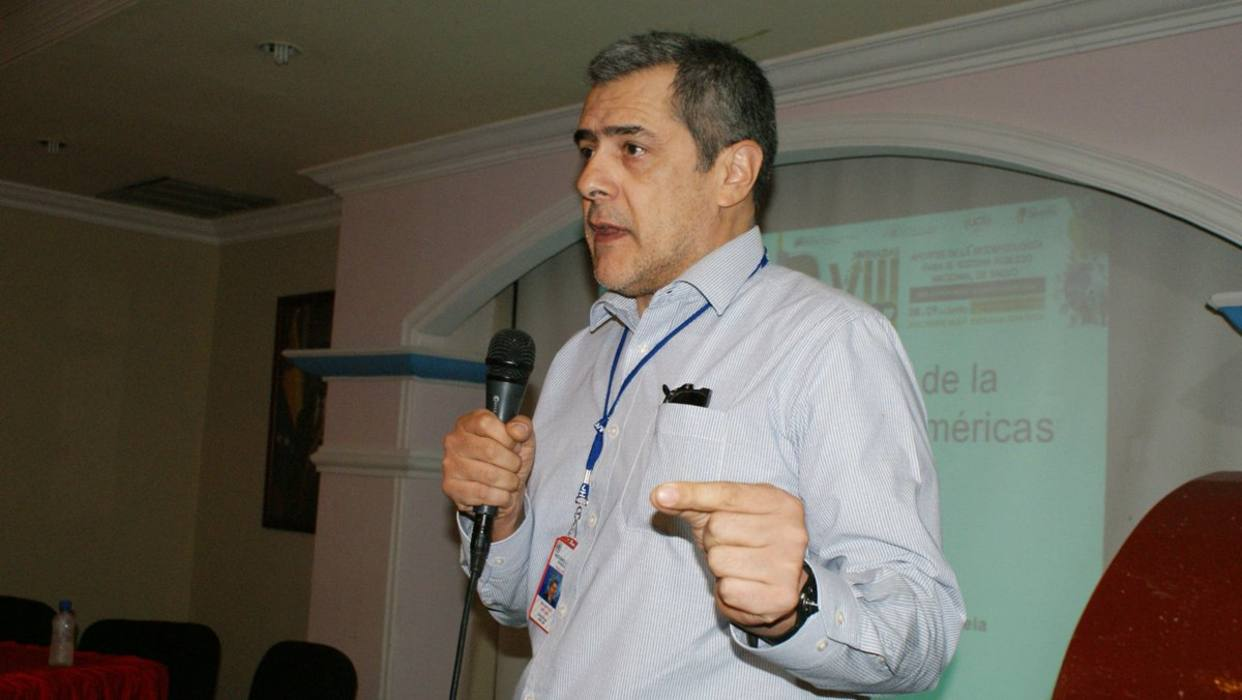
\includegraphics[width=300px]{114.jpg}%
\newline%
%
El Plan Maestro elaborado por la Organización Panamericana de la Salud/Organización Mundial de la Salud junto con el Ministerio de Salud, para fortalecer la respuesta frente al VIH/Sida, la tuberculosis y la malaria en el país, fue aprobado para que se realice a comienzos del año 2019. José Moya, representante de las citadas organizaciones en Venezuela, presentó ayer en el foro~VIH en el contexto de la emergencia humanitaria, un adelanto de las medidas que se tomarán con esta estrategia que ya cuenta con 5 millones de dólares aprobados para la compra de medicamentos y tratamientos a fin de combatir esas enfermedades en el país.%
\newline%
%
El documento, aseguró Moya, fue sometido al Fondo Global que finalmente aprobó 5 millones de dólares para apoyarlo, una cantidad que se dispuso para las órdenes de compra de fármacos.%
\newline%
%
“El Plan Maestro se proyecta a tres años y cuenta con un monto cercano a los 122 millones de dólares. Es fundamental planificar con anticipación las necesidades de medicinas, pruebas de diagnóstico e insumos de laboratorio”, expuso.%
\newline%
%
“Venezuela está considerada como un país con altos ingresos, por eso no califica para la ayuda del Fondo Global, sin embargo, se hicieron gestiones y este año, luego de mucho trabajo por parte de la sociedad civil, el fondo abrió sus puertas y finalmente se aprobó la ayuda”, señaló.%
\newline%
%
El documento, indicó Moya, se elaboró junto con expertos de la OPS, la sociedad civil, infectólogos, funcionarios del Ministerio de Salud y “todas las personas involucradas en dar respuesta a las tres enfermedades en conocimiento, diagnóstico y análisis”. El trabajo expone la situación en términos de disponibilidad de medicamentos, insumos de laboratorios, reactivos, necesidades y todo aquello para trabajar en respuestas.%
\newline%
%
Uno de los temas principales del plan, aseveró Moya, es asegurar la existencia de fármacos para enfermedades crónicas: “Sabemos que durante meses ha habido discontinuidad en los tratamientos y sabemos el impacto que eso produce en las personas que los necesitan”.%
\newline%
%
VIH: Emergencia humanitaria%
\newline%
%
En el foro en el que participaron organizaciones como Acción Ciudadana contra el Sida, Red Venezolana de Gente Positiva, David, Mujeres en Línea, ONUSida, Asociación Civil VIH y Arcoiris por la Vida, se expuso el delicado estatus en el que se encuentra el sector salud en Venezuela y, principalmente, el estado de los afectados por la crisis. Eduardo Franco, secretario de RVG+ denunció que no se están cumpliendo los artículos 83 y 84 de la Constitución: “En Venezuela no se cumple el derecho a la vida, los familiares también están aquejados”. Además, denunció la reaparición de la enfermedad sarcoma de Kaposi por la falta de medicamentos así como la discriminación que padecen las personas con VIH.%
\newline%
%
Alberto Nieves declaró que actualmente en el país hay un retraso fuerte en la medicación del VIH: “Los antirretrovirales no llegan a los estómagos de las personas”, dijo, y recordó que desde 2016 el gobierno no ha publicado cifras oficiales sobre la enfermedad. “El Estado no reconoce el desabastecimiento de medicamentos”, recalcó.%
\newline%
%
\end{document}